% Chapter 5 --- Mechanical Innovation and Granular Dispersion

\chapter{Mechanical Innovation and Granular Dispersion}\doublespacing
\label{Chapter5}
\lhead{Chapter IV. \emph{Mechanical Innovation and Granular Dispersion}}

%----------------------------------------------------------------------------------------
\section{The Necessity of Mechanical Dispersion}
%----------------------------------------------------------------------------------------

The insight that came out of Prototype II was simple to state and took some time to fully absorb: before the system can classify grains, it has to see them. A top-view camera looking down at a dense, three-dimensional pile of 2,800 wheat entities does not have clear sight of most of them. The entities on the exposed surface are imaged; the others are not. Any $W/W\%$ estimate derived from those visible-surface images alone is, in effect, a statistical guess---it might be accurate on average, or it might not, depending on whether the sample has settled in a representative configuration.

For reliable quality assessment, grains need to be presented to the camera progressively: different specimens visible in different frames, different surfaces of each specimen exposed across a capture sequence. This requires two distinct forms of physical motion. \textit{Lateral dispersion} reduces overlap and moves buried grains to the surface. \textit{Rotational excitation} varies grain orientation so that defect signatures on non-top surfaces---the ventral marks of \textit{Infested} grain, the peripheral darkening of \textit{Black Tip}---are captured in at least some frames. Neither optical filtering nor algorithmic improvement can substitute for this; the information has to enter the imaging system in the first place.

The question was how to generate both types of motion reliably, repeatedly, and without damaging the grain in the process.

%----------------------------------------------------------------------------------------
\section{Failure Analysis: Vibratory Agitation}
%----------------------------------------------------------------------------------------

Vibration was the obvious first candidate. It is widely used in grain handling equipment, the implementation is straightforward, and the hardware cost is modest. Several vibration motor configurations were evaluated---low-, medium-, and high-torque units, at different mounting positions and drive frequencies.

The results were discouraging in three specific ways.

The first problem was what might be called \textit{contact impedance}: the transfer of motor energy to the grain surface was uneven. Variable coupling between motor and tray, combined with changing load distribution as grain redistributed during agitation, created spatial dead zones where grains moved minimally regardless of drive level. Increasing motor torque exacerbated this, tending to produce energetic motion at the tray periphery while the central pile remained relatively static.

The second problem was more fundamental: prolonged vibration produced size-based segregation effects consistent with what the granular physics literature describes as the Brazil Nut Effect \cite{Rosato1987, Ottino2000}. Under repetitive vibration, denser or smaller particles---in this context, stones, earth balls, and fine impurities---migrate downward, while larger or lighter fractions accumulate near the exposed surface \cite{SizeSegregation2021}. For a quality assessment system, this is an actively bad property. The camera ends up over-sampling the upper grain layer, which becomes progressively less representative of the sample's true composition. The estimate that results is biased in a direction that happens to make the batch appear cleaner than it is.

The third problem was limited rotational excitation. Vibration generated primarily in-plane grain motion; out-of-plane flipping---which is what exposes non-top grain surfaces---was rare and not controllable. Grain shuffled, but did not turn over.

Vibration was therefore set aside. The question became: what kind of motion, and what kind of actuation mechanism, could produce consistent lateral dispersion and rotational excitation without the segregation effects?

%----------------------------------------------------------------------------------------
\section{Electromagnetic Solenoid Actuation}
%----------------------------------------------------------------------------------------

The answer emerged from a change in framing. Instead of continuous oscillation, the mechanism needed to deliver discrete, high-energy impulses---brief events that break local grain packing and induce rotation, separated by resting intervals during which the grain bed settles before the next impulse. This is mechanically quite different from vibration: less continuous energy, higher instantaneous force, and a fundamentally different motion character.

Electromagnetic solenoids suited this requirement. On activation, a solenoid drives its plunger through a defined stroke in a few milliseconds, delivering a concentrated impact to whatever is in contact with the plunger tip. On deactivation, it retracts under a return spring. The force profile is sharp and localised, generating upward acceleration that is more effective at inducing grain rotation than the lateral-dominant motion of vibration.

The tray was coupled to four solenoids positioned at the cardinal midpoints of its underside, oriented to deliver distributed vertical impulses across the full imaging area. The arrangement was chosen to avoid having all impulse energy concentrated in one region of the tray.

\begin{figure}[H]
    \centering
    \begin{subfigure}[t]{0.48\textwidth}
        \centering
        \includegraphics[width=\textwidth]{before solenoid action.png}
        \caption{Before dispersion: dense, multi-layered packing with significant occlusion.}
        \label{fig:before_solenoid}
    \end{subfigure}
    \hfill
    \begin{subfigure}[t]{0.48\textwidth}
        \centering
        \includegraphics[width=\textwidth]{after solenoid action.png}
        \caption{After dispersion: measurable grain isolation and orientation diversity following a single actuation cycle.}
        \label{fig:after_solenoid}
    \end{subfigure}
    \caption{The 100-gram grain sample before and after a single solenoid actuation cycle, demonstrating the transition from dense occlusion to measurable grain isolation and orientation diversity.}
    \label{fig:solenoid_dispersion}
\end{figure}

%----------------------------------------------------------------------------------------
\section{Asynchronous Pulse Logic and Timing}
%----------------------------------------------------------------------------------------

Firing all four solenoids simultaneously introduced a new problem. Coincident plunger impacts sent constructive and destructive wave fronts through the tray simultaneously, producing irregular and sometimes violently uneven grain motion, including occasional ejection of grain from the tray boundary---not acceptable in a system that is supposed to be quantifying a 100-gram sample.

The solution was asynchronous sequencing. By staggering solenoid activation in series, each impulse was allowed to propagate through the grain bed before the next began. The result was a travelling shear wave that was effective for both de-clumping and rotation in a way that simultaneous firing was not.

Using Raspberry Pi 5 GPIO control, with solenoids $\{S_A, S_B, S_C, S_D\}$, activation timing was structured as follows:

\begin{align}
    T_A &= t \nonumber \\
    T_B &= t + 50\,\text{ms} \nonumber \\
    T_C &= t + 100\,\text{ms} \nonumber \\
    T_D &= t + 150\,\text{ms}
    \label{eq:solenoid_timing}
\end{align}

Each solenoid deactivates 500\,ms after activation; one complete cycle therefore spans 650\,ms. The 50\,ms inter-solenoid interval was arrived at empirically: intervals below 40\,ms began to reintroduce interference effects, while intervals above 80\,ms weakened the cross-tray shear action that made this approach effective. Multiple cycles are executed per assessment session, with image capture interleaved between cycles to accumulate orientation diversity across the full frame sequence.

\begin{figure}[H]
    \centering
    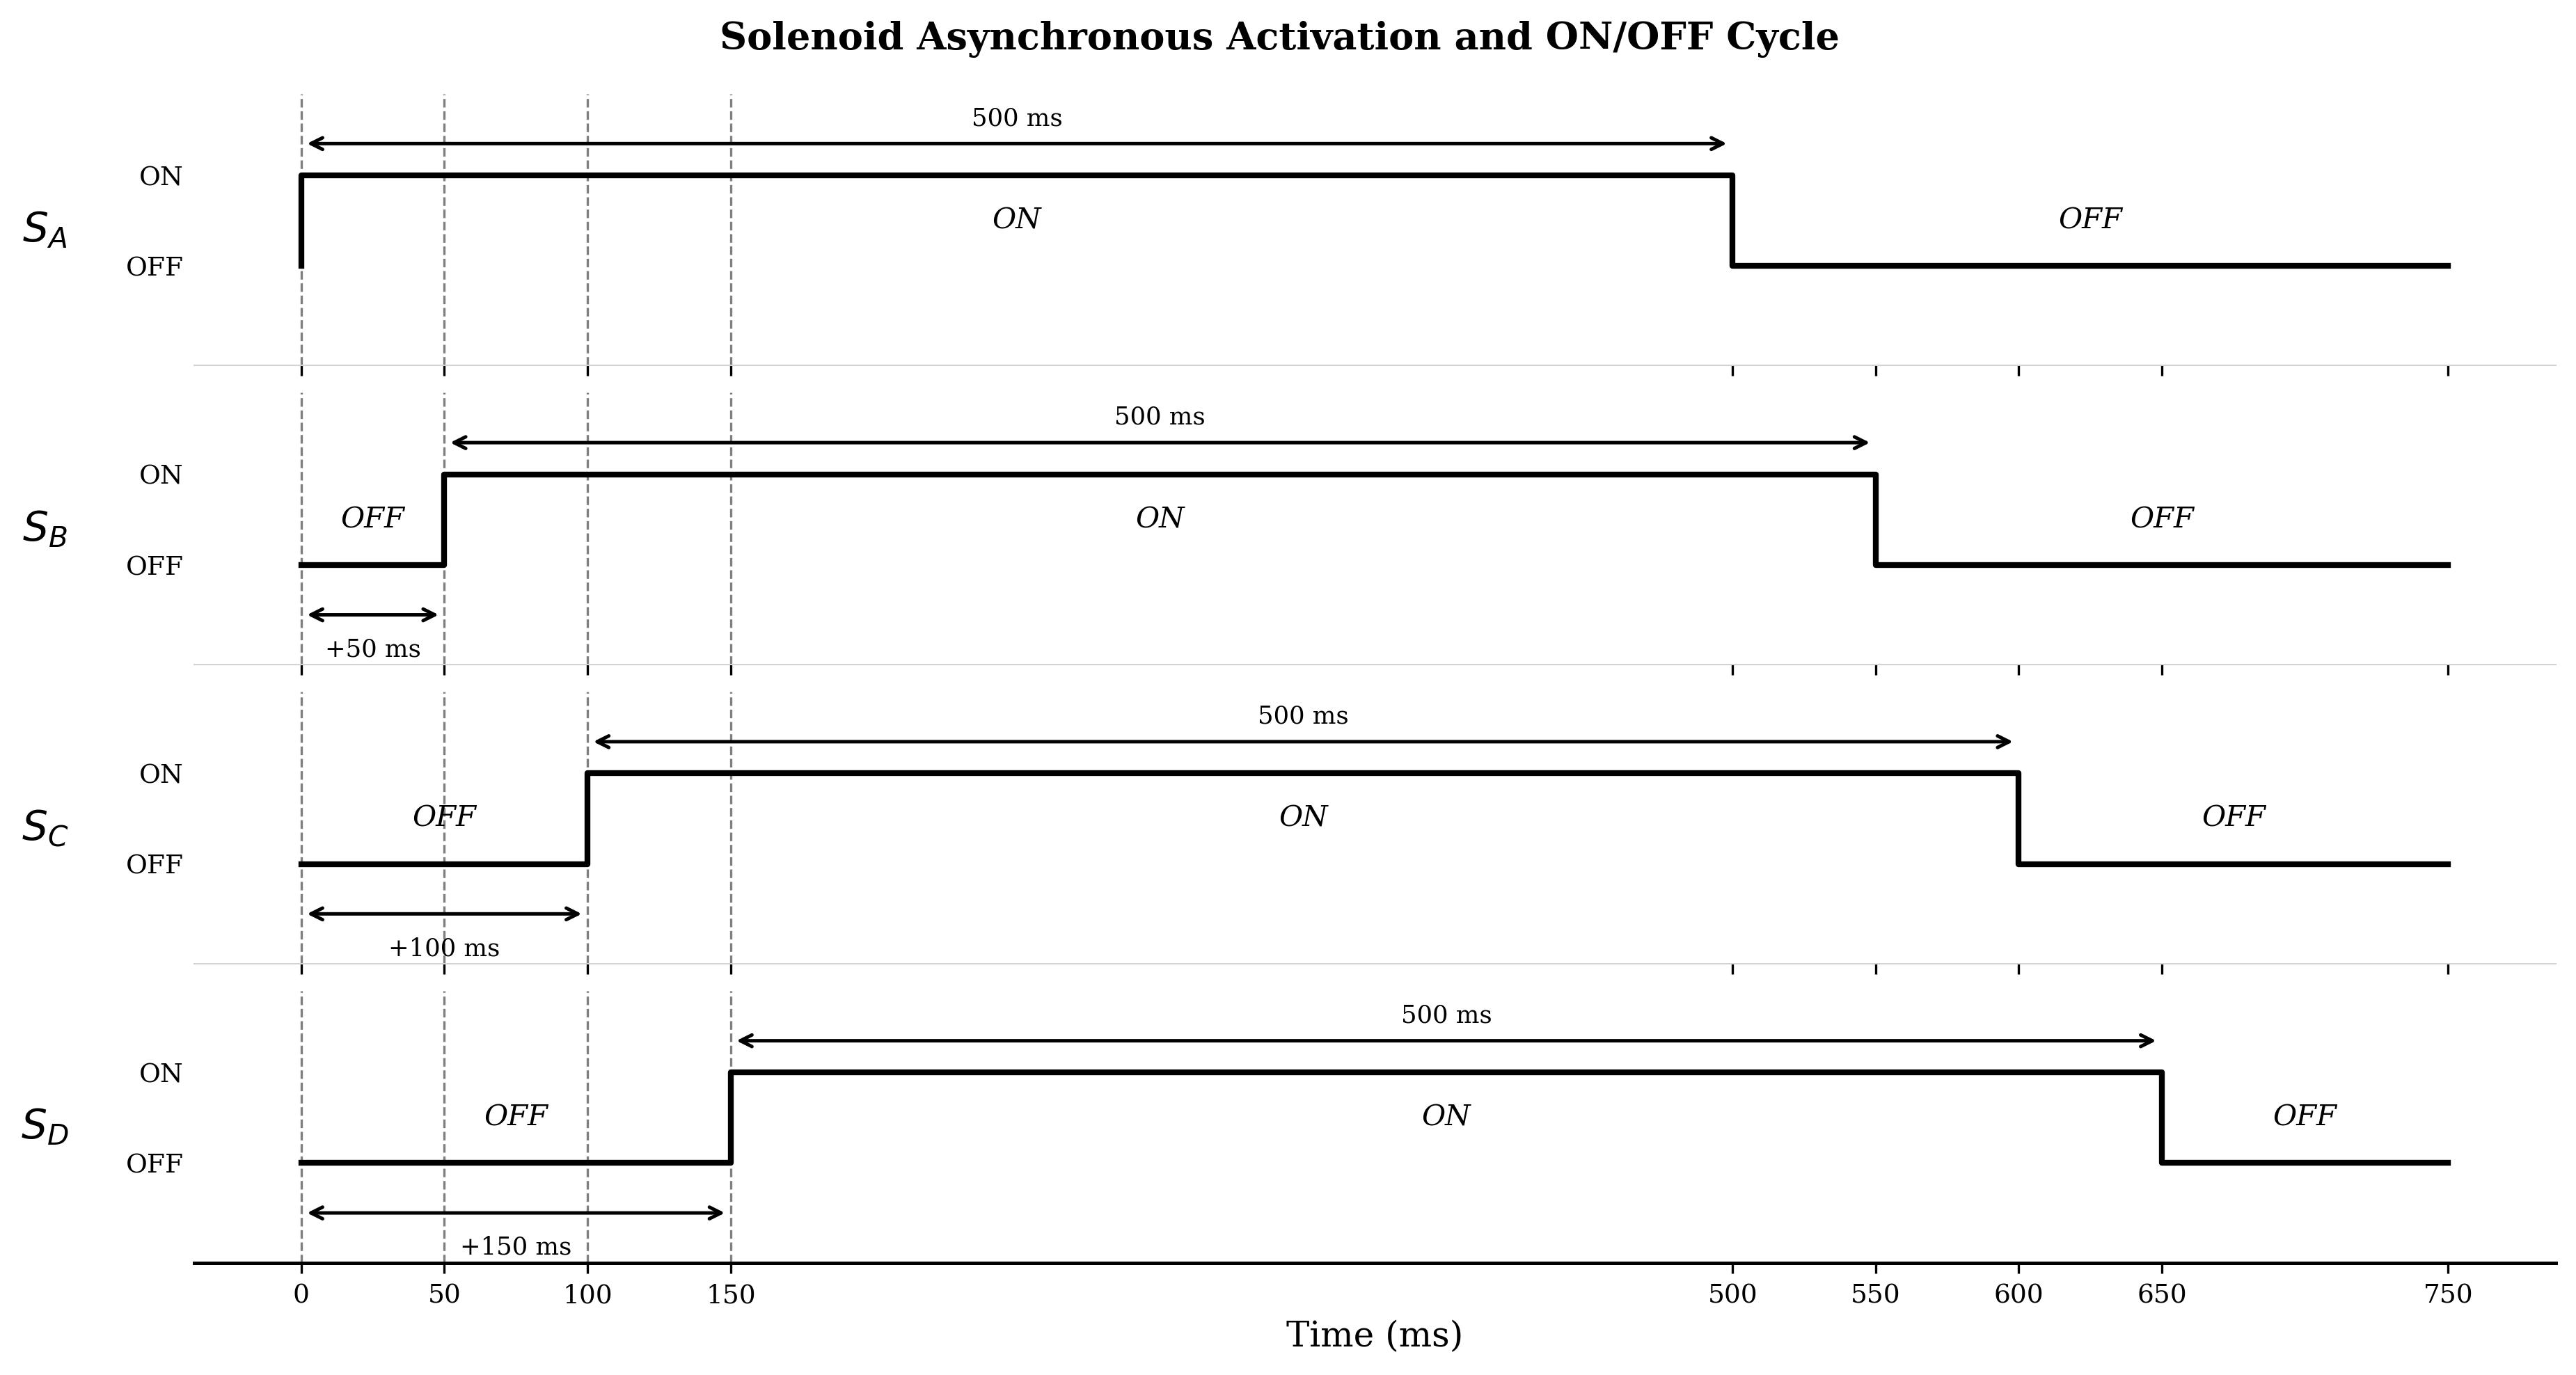
\includegraphics[width=0.95\textwidth]{Images/solenoid_timing.png}
    \caption{Timing diagram for the staggered asynchronous solenoid pulse protocol. Each solenoid ($S_A$ through $S_D$) activates sequentially with a 50\,ms inter-solenoid delay and remains active for 500\,ms. The complete four-solenoid cycle spans 650\,ms. The staggered pattern produces a travelling impulse wave across the tray, generating grain rotation and dispersion without interference between simultaneous activations.}
    \label{fig:solenoid_timing}
\end{figure}

%----------------------------------------------------------------------------------------
\section{Hardware Integration: The Hole-Fitting Mechanism}
%----------------------------------------------------------------------------------------

Having settled on solenoid actuation, the remaining design problem was the mechanical interface between the solenoid plungers and the sample tray. Poor coupling at this interface---any compliance, flex, or friction that absorbs part of the plunger stroke---converts a sharp impulse into a damped vibration. The grain bed responds accordingly: reduced de-clumping, reduced rotation, reduced diversity of captured orientations.

Two interface approaches were explored.

The first was a \textbf{drawer mechanism}: a pull-out tray on guide rails with magnetic retention. The ergonomic logic was reasonable---drawer mechanisms are familiar and reduce the cognitive overhead of loading a sample. In practice, it failed for two reasons. Magnetic retention was destabilised by the active solenoid magnetic fields, producing inconsistent retention force that was difficult to characterise and impossible to make reliable under all operating conditions. More critically, the guide rails introduced flex and friction that absorbed significant plunger energy, effectively undoing the impulse actuation strategy.

The second approach, which became the final design, was a \textbf{hole-fitting mechanism}: the tray has four precision apertures positioned to align with the solenoid plungers when the tray is seated. Plungers engage directly through the apertures on activation, creating near-rigid force transfer with minimal damping. The tray is loaded by placing it vertically onto the plunger array---a motion that is slightly less immediately intuitive than a drawer pull, but one that takes less than two seconds to perform and proved entirely unproblematic in user observation during the Bangalore demonstration.

The same design simplified maintenance. Tray removal and replacement requires only vertical motion---no rails to accumulate dust blockages, no fasteners, no tools.

%----------------------------------------------------------------------------------------
\section{Summary}
%----------------------------------------------------------------------------------------

The mechanical development described in this chapter is largely a record of following failure to its source. Vibration failed specifically---not generically---in ways that illuminated exactly what the dispersion mechanism needed to do differently. Solenoid impulse actuation with staggered timing addressed each of those failure modes directly, and the hole-fitting tray interface ensured that the energy intended for the grain bed actually reached it. The system that resulted converts a physically intractable dense-pile imaging problem into a tractable sequence-of-frames classification problem by making the required information enter the camera over time. Chapter~\ref{Chapter6} describes what happens to that information once it does.

%----------------------------------------------------------------------------------------
\section{Final Hardware Integration and Prototyping}
%----------------------------------------------------------------------------------------

With each subsystem validated independently---optoelectrical calibration, solenoid actuation, tray interface---the final stage was assembly of the high-fidelity prototype. This was not simply a matter of combining components. The spatial relationships between the solenoid array, the imaging surface, the LCD backlight, and the camera mount were all constrained by the impulse mechanics; if the tray moved too far from the camera focal plane under actuation, image sharpness would degrade during the most informative capture moments.

Figure~\ref{fig:final_integration} documents the physical assembly sequence: custom PCB fabrication, chassis assembly around the solenoid array, wiring, and the fully assembled device. The custom PCB consolidated solenoid driver circuits and GPIO timing into a single board, replacing a prototype breadboard arrangement that had proven unreliable in conditions of dust and physical vibration.

\begin{figure}[p]
    \centering
    \includegraphics[width=\textwidth,height=0.85\textheight,keepaspectratio]{final CAD exploded view.PNG}
    \caption{CAD exploded view of the Drishti device, showing the vertical component stack: optics module, electromagnetic actuation array, and control electronics within the aluminium chassis.}
    \label{fig:final_cad_full}
\end{figure}

\begin{figure}[H]
    \centering
    % Row 1: 3 images
    \begin{subfigure}[t]{0.32\textwidth}
        \centering
        
\includegraphics[width=\textwidth]{final PCB circuit.jpg}
        \caption{Custom PCB.}
        \label{fig:final_pcb}
    \end{subfigure}
    \hfill
    \begin{subfigure}[t]{0.32\textwidth}
        \centering
        
\includegraphics[width=\textwidth]{final prototype making 1.jpg}
        \caption{Chassis assembly.}
        \label{fig:final_proto_1}
    \end{subfigure}
    \hfill
    \begin{subfigure}[t]{0.32\textwidth}
        \centering
        
\includegraphics[width=\textwidth]{final prototype making 2.jpg}
        \caption{Solenoid mounting.}
        \label{fig:final_proto_2}
    \end{subfigure}
    
    \vspace{2em}
    
    % Row 2: 2 images, centered
    \begin{subfigure}[t]{0.32\textwidth}
        \centering
        
\includegraphics[width=\textwidth]{final prototype making 3.jpg}
        \caption{Hardware wiring.}
        \label{fig:final_proto_3}
    \end{subfigure}
    \hspace{0.05\textwidth}
    \begin{subfigure}[t]{0.32\textwidth}
        \centering
        
\includegraphics[width=\textwidth]{final prototype photo.jpg}
        \caption{Fully assembled.}
        \label{fig:final_proto_photo}
    \end{subfigure}

    \caption{Physical assembly sequence of the final prototype. (a)~Custom PCB for solenoid pulse timing. (b--d)~Progressive chassis and electronics assembly. (e)~Completed device prepared for deployment.}
    \label{fig:final_integration}
\end{figure}
